% !TEX root=ricardo_draft.tex
\begin{figure}[!th]
\begin{center}
\vspace{-1ex}
\centerline{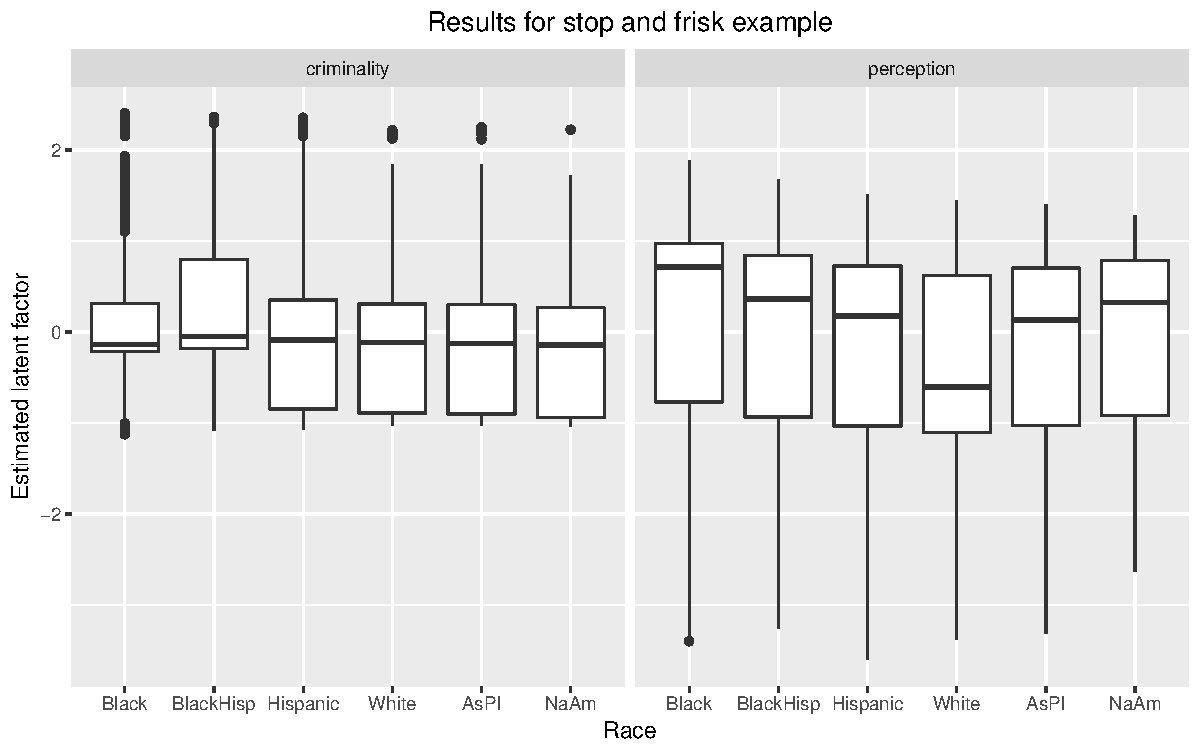
\includegraphics[width=\columnwidth]{stopandfrisk_output.pdf}}
\vspace{-2ex}
\caption{Distributions of estimated latent perception and criminality scores for the stop and frisk dataset.\label{figure.stop_and_frisk_output}}
\vspace{-2ex}
\end{center}
\end{figure}

In this section we evaluate our framework for modeling fairness. We test our approach on two practical problems in which fairness must be enforced. For each problem we construct causal models, and make explicit how unfairness may affect observed and unobserved variables in the world. Given these models we are able to (a) derive counterfactually fair predictors and (b) predict latent variables such as a person's `criminality' (which may be useful for predicting crime) as well as their `perceived criminality' (which may be due to prejudices based on race and gender). Additionally, we can analyze how realistic our models are by comparing our observations with data generated from the model. We consider two real-world problems, the first is \emph{fair prediction of success in law school} and the second is \emph{separating actual and perceived criminality in stop-and-frisk data}.

\subsection{Law school success}
Between the years of 1991-1996 the Law School Admission Council
counducted a longitudinal survey following students across 163 law
schools in the United States \cite{wightman1998lsac}. The survey was
designed to assess `the law school experience of minority students, as
well as their ultimate entry into the profession'. The survey contains
students' features before entering law school including: their
entrance exam (LSAT) scores and their undergraduate grade-point
average (GPA); features from during law school, such as, their average
grade of their first-year of law school (FYA)), and following Law
School i.e. whether students passed the final examination, the `bar
exam' (P)).

Given this data a law school may wish to predict whether a law student
will pass the final bar exam from information about their performance
during and before law school. The school would also like to make sure
these predictions are not biased by an individual's race and
gender. However, we may worry that our observed information about
students, the LSAT, GPA, and FYA scores, are biased due to historical
social factors relating to race and gender. Our approach is to model these
``unfair'' factors as well as a latent variable that is counterfactually
fair. We will then be able to use this latent variable as a feature
for prediction.

We propose to model the law school data as shown in
Figure~\ref{figure.law_school}. We suspect that variables race and sex
affect student performance (e.g. GPA, LSAT, and FGA) due to factors
such as cultural norms, which assume that individuals of a certain
race or gender are `better suited' to be lawyers. Such beliefs could
adversely impact students who do not fit these norms. Instead we would
like to model the latent \emph{knowledge} (K) of a student, which also
impacts these features as well as whether the student passes their
final bar exam (P). We can then construct a predictor $\hat{Y}$ that
predicts P fairly using knowledge and the testing location (LOC) which
we suspect may have an affect on P. It is easy to show that $\hat{Y}$
is counterfactually fair, whereas a predictor that uses features GPA,
LSAT, and FGA is not (in this case even including race and sex as
features cannot correct this, as can be done in the linear case). The
causal model is a short-hand for a system of equations:
\begin{align}
G &\sim {\cal N}(b_G + w_1 K + w_2 R + w_3 S, \sigma_G) \nonumber \\
L &\sim \textrm{Poisson}(\exp(b_L + w_4 K + w_5 R + w_6 S)) \nonumber \\
F &\sim {\cal N}(b_F + w_7 K + w_8 R + w_{9} S, 1) \nonumber \\
P &\sim \textrm{Bernoulli}([1+\exp(-b_P + w_{10} K + w_{11} R + w_{12} S)]^{-1}) \nonumber \\
K &\sim {\cal N}(0,1) \nonumber
\end{align}

 

% TODO rank top 10 students by ability or by other score in law_school.py which only considers observed features
\begin{figure*}[th]
\begin{center}
\vspace{-2ex}
\centerline{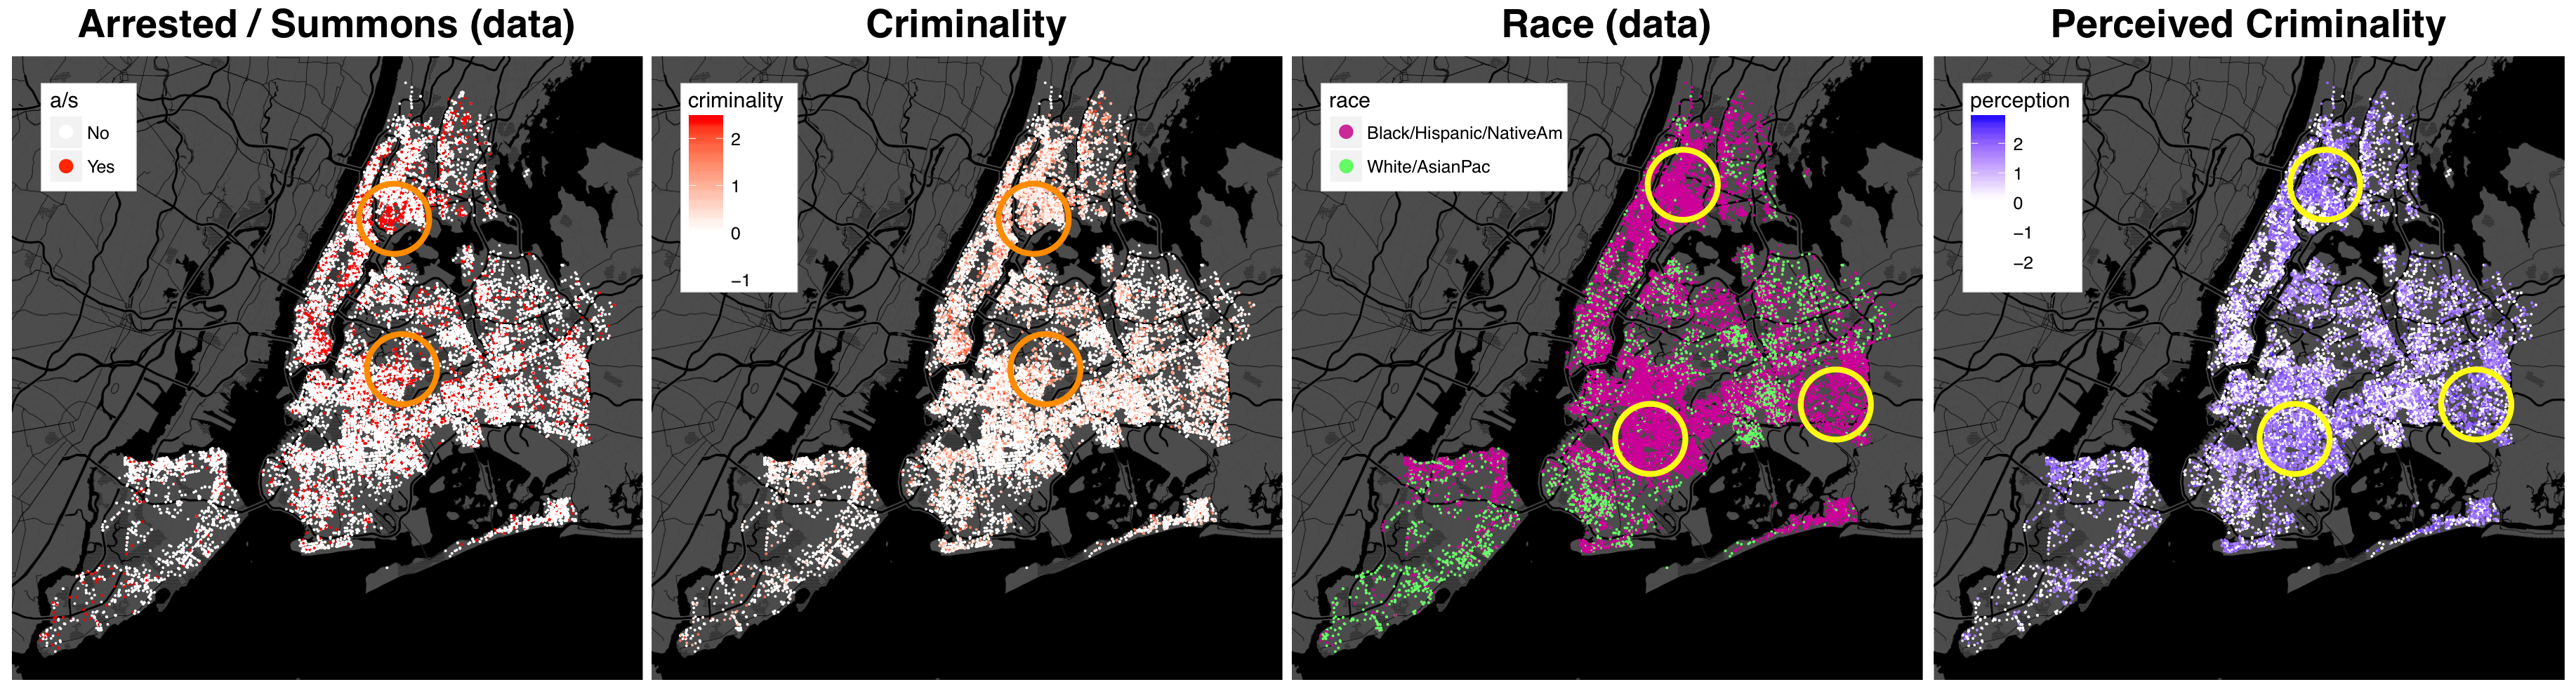
\includegraphics[width=\textwidth]{stop_and_frisk_graphs.png}}
\vspace{-2ex}
\caption{P.}
\label{figure.criminality}
\vspace{-2ex}
\end{center}
\end{figure*}

\begin{figure}[th]
\begin{center}
\vspace{-1ex}
\centerline{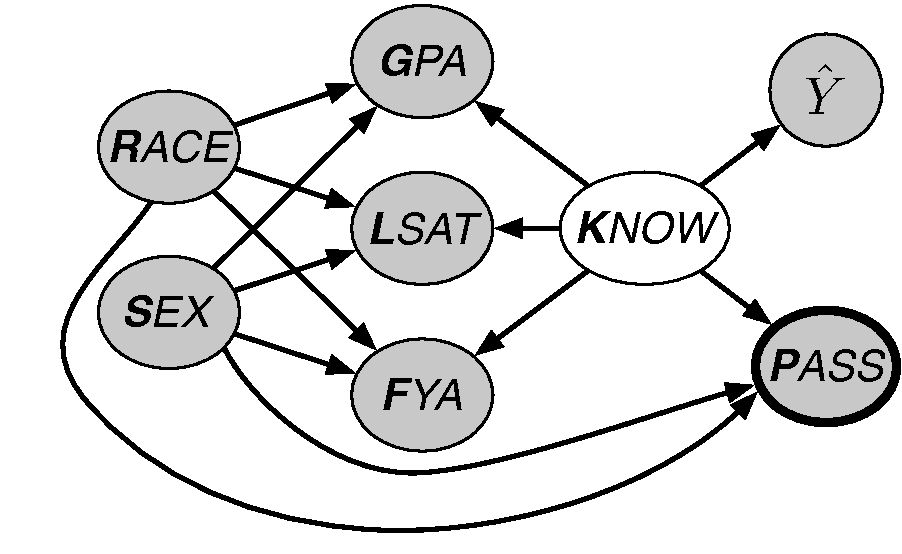
\includegraphics[width=\columnwidth]{law_school_model}}
\vspace{-2ex}
\caption{A causal model for the problem of predicting law school success fairly.\label{figure.law_school}}
\vspace{-2ex}
\end{center}
\end{figure}

\begin{table}[t]
\vspace{-2ex}
\caption{Prediction results using logistic regression. Note that we must sacrifice a small amount of accuracy to ensuring counterfactually fair prediction (fair), versus the model which uses all features, including race and sex (unfair).}
\vspace{-3ex}
\label{table.pred_law}
\begin{center}
\resizebox{\columnwidth}{!}
{
\begin{sc}
\footnotesize
\begin{tabular}{c|c|c}
\hline
%\multicolumn{5}{c}{\textbf{Lower Bounds}}\\
\hline
model & balanced acc. & F1-score  \\
\hline
unfair & 0.590 & 0.293 \\ \hline
fair  &  0.562 & 0.216 \\
\hline
\end{tabular}
\end{sc}
}
\end{center}
\vspace{-4ex}
\end{table}


\subsection{True vs. Perceived Criminality}
Every year since 2002, the New York Police Department (NYPD) has recorded information about every time a police officer has stopped someone. The officer records information such as if they searched or frisked the individual, whether a weapon was found, the individual's appearance, whether force was used, etc. We look at this data collected during 2014 for our analysis.


\begin{figure}[th]
\begin{center}
\vspace{-1ex}
\centerline{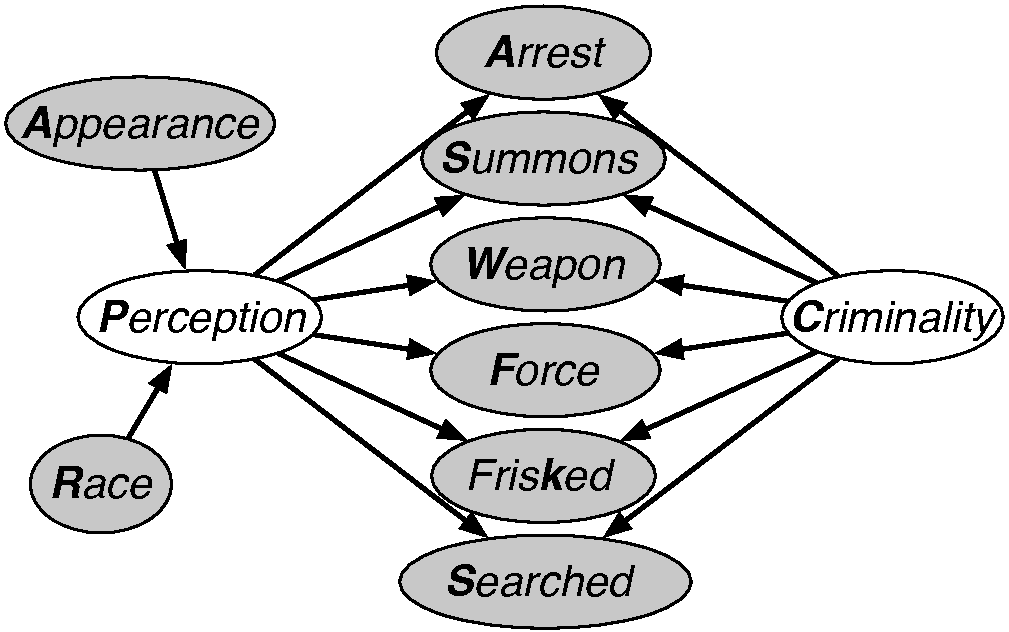
\includegraphics[width=\columnwidth]{stop_and_frisk_model3.pdf}}
\vspace{-2ex}
\caption{A causal model for the stop and frisk dataset.\label{figure.stop_and_frisk}}
\vspace{-2ex}
\end{center}
\end{figure}


\subsection{Model criticism}
%%% Local Variables:
%%% mode: latex
%%% TeX-master: "ricardo_draft"
%%% End:
